\documentclass[11pt]{article}
\usepackage{amsmath, amssymb}
\usepackage[margin=1in]{geometry}
\usepackage{booktabs}
\usepackage{pgfplots}
\pgfplotsset{compat=1.18}
\usepackage{tikz}

\newcommand{\R}{\mathbb{R}}

\title{DoG Scale Bias: Why Detected $\sigma$ Underestimates True Blob Scale}
\author{BlobBoards Technical Note}
\date{}

\begin{document}
\maketitle

\section{Setup}

Consider a 2D isotropic Gaussian blob centered at the origin with scale
$\sigma_b$:
\begin{equation}
  I(\mathbf{x}) = A \exp\!\Bigl(-\frac{|\mathbf{x}|^2}{2\sigma_b^2}\Bigr).
\end{equation}
The scale space is built by convolving with Gaussians of increasing scale
$\sigma$. At cumulative smoothing scale~$\sigma$, the image value at the
center is:
\begin{equation}
  I_\sigma(\mathbf{0})
    = A \,\frac{\sigma_b^2}{\sigma_b^2 + \sigma^2}.
  \label{eq:smoothed-center}
\end{equation}

\section{Difference of Gaussians}

The scale space is sampled at discrete scales with constant ratio
$k = 2^{1/S}$, where $S$ is the number of subdivisions per octave
(typically $S=3$, giving $k \approx 1.26$).

The Difference of Gaussians (DoG) at level~$s$ is:
\begin{equation}
  D_s = G_{k\sigma_s} * I - G_{\sigma_s} * I,
\end{equation}
where $\sigma_s$ is the cumulative smoothing scale at subdivision~$s$.

At the blob center, the DoG response is:
\begin{equation}
  D_s(\mathbf{0})
    = A\,\sigma_b^2
      \left[
        \frac{1}{\sigma_b^2 + k^2\sigma_s^2}
        - \frac{1}{\sigma_b^2 + \sigma_s^2}
      \right].
  \label{eq:dog-center}
\end{equation}

\section{Peak Location}

To find where the DoG response peaks as a function of $\sigma_s$, we
differentiate~\eqref{eq:dog-center} with respect to $\sigma_s$ and set it
to zero:
\begin{equation}
  \frac{\partial}{\partial \sigma_s} D_s(\mathbf{0})
    = A\,\sigma_b^2
      \left[
        \frac{2\sigma_s}{(\sigma_b^2 + \sigma_s^2)^2}
        - \frac{2k^2\sigma_s}{(\sigma_b^2 + k^2\sigma_s^2)^2}
      \right]
    = 0.
\end{equation}
Dividing by $2\sigma_s$ (assuming $\sigma_s > 0$):
\begin{equation}
  \frac{1}{(\sigma_b^2 + \sigma_s^2)^2}
    = \frac{k^2}{(\sigma_b^2 + k^2\sigma_s^2)^2}.
\end{equation}
Taking the positive square root:
\begin{equation}
  \frac{1}{\sigma_b^2 + \sigma_s^2}
    = \frac{k}{\sigma_b^2 + k^2\sigma_s^2}.
\end{equation}
Cross-multiplying:
\begin{equation}
  \sigma_b^2 + k^2\sigma_s^2 = k\,(\sigma_b^2 + \sigma_s^2)
  \quad\Longrightarrow\quad
  \sigma_b^2(1 - k) = \sigma_s^2(k - k^2) = -k\,\sigma_s^2(k - 1).
\end{equation}
Therefore:
\begin{equation}
  \boxed{\sigma_s^{\star} = \frac{\sigma_b}{\sqrt{k}}}
  \label{eq:peak}
\end{equation}

\section{The Bias}

The DoG response for a blob of true scale $\sigma_b$ peaks at the scale
level where the \emph{lower} Gaussian has scale
$\sigma_s^\star = \sigma_b / \sqrt{k}$.

If we assign $\sigma_s$ (the lower Gaussian scale) as the detected scale,
we get:
\begin{equation}
  \sigma_{\text{detected}} = \sigma_s^\star = \frac{\sigma_b}{\sqrt{k}}.
\end{equation}
The ratio is:
\begin{equation}
  \frac{\sigma_{\text{detected}}}{\sigma_b} = \frac{1}{\sqrt{k}}
    = 2^{-1/(2S)}.
\end{equation}

\begin{table}[h]
\centering
\begin{tabular}{@{}ccc@{}}
\toprule
$S$ & $k = 2^{1/S}$ & $1/\sqrt{k}$ \\
\midrule
2 & 1.4142 & 0.8409 \\
3 & 1.2599 & 0.8909 \\
4 & 1.1892 & 0.9170 \\
5 & 1.1487 & 0.9330 \\
\bottomrule
\end{tabular}
\caption{Scale underestimation factor for different octave resolutions.
For $S=3$, the detected scale is $\approx 89\%$ of the true scale.}
\end{table}

\noindent
Subpixel refinement does \emph{not} fix this.  Refinement finds the peak
location more precisely, but the mapping from scale-space index to
$\sigma$ is calibrated to the lower Gaussian.  A perfectly precise peak
location still reads off $\sigma_b / \sqrt{k}$.

\section{The Fix}

The characteristic scale of the DoG filter between $G(\sigma_s)$ and
$G(k\sigma_s)$ is the geometric mean:
\begin{equation}
  \sigma_{\text{char}} = \sqrt{\sigma_s \cdot k\sigma_s} = \sigma_s\sqrt{k}.
\end{equation}
If we assign $\sigma_{\text{char}}$ instead of $\sigma_s$ to each DoG
level, the bias vanishes:
\begin{equation}
  \sigma_{\text{detected}} = \sigma_s^\star \cdot \sqrt{k}
    = \frac{\sigma_b}{\sqrt{k}} \cdot \sqrt{k} = \sigma_b.
\end{equation}

In the code, the correction is applied when converting scale-space extrema
to detections. The scale-space internals retain the standard lower-sigma
convention (consistent with VLFeat/SIFT), and the $\sqrt{k}$ factor is
applied as a post-hoc correction using the known octave resolution~$S$:
\begin{verbatim}
  sqrt_k = 2.0^(1.0 / (2 * octave_resolution))
  detection.sigma = extremum.sigma * sqrt_k
\end{verbatim}

\section{Crowding Bias in Dense Patterns}

After applying the $\sqrt{k}$ correction, isolated blobs are detected at
their true scale (ratio $\approx 1.000$). However, in dense blob patterns
a \emph{residual} underestimation remains that depends on the inter-blob
spacing.  Empirically:

\begin{table}[h]
\centering
\begin{tabular}{@{}cccc@{}}
\toprule
Render extent & Blob count & Median $\sigma_{\det}/\sigma_b$ & Std \\
\midrule
$2\sigma$ & 468 & 0.843 & 0.035 \\
$3\sigma$ & 238 & 0.985 & 0.012 \\
$4\sigma$ & 185 & 0.998 & 0.004 \\
Isolated  &   1 & 1.000 & --- \\
\bottomrule
\end{tabular}
\caption{Scale accuracy after $\sqrt{k}$ correction. Denser packing
(smaller render extent) causes additional underestimation.}
\end{table}

\subsection{Mexican hat interpretation}

The DoG approximates the Laplacian of Gaussian (LoG), which acts as a
\emph{Mexican hat} operator: a positive center lobe of width $\sim\!\sigma$
surrounded by a negative annulus extending to $\sim\!2$--$3\sigma$.  The
response at a blob center equals the contrast between the average intensity
under the center lobe and the average intensity under the surround annulus.

\begin{figure}[h]
\centering
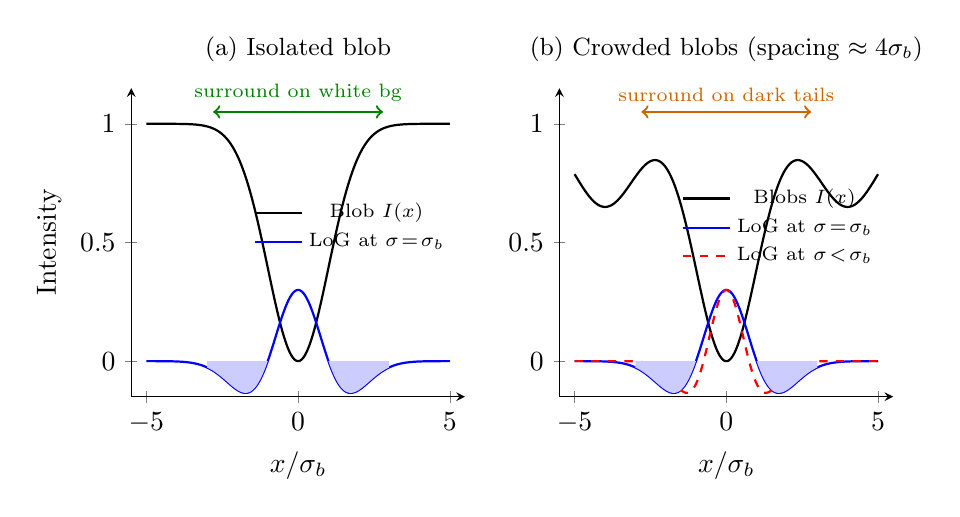
\begin{tikzpicture}
\begin{axis}[
  name=plotA,
  width=0.48\textwidth, height=5.5cm,
  title={\small (a) Isolated blob},
  xlabel={$x / \sigma_b$},
  ylabel={Intensity},
  xmin=-5.5, xmax=5.5,
  ymin=-0.15, ymax=1.15,
  ytick={0, 0.5, 1.0},
  axis lines=left,
  clip=false,
  legend style={at={(0.98,0.55)}, anchor=east, font=\scriptsize,
                draw=none, fill=none},
]
% Blob profile: 1 - exp(-x^2/2)
\addplot[black, thick, domain=-5:5, samples=200]
  {1 - exp(-x^2/2)};
\addlegendentry{Blob $I(x)$}

% LoG at matched scale (sigma=1), scaled and shifted for visibility
% LoG(x;s) = (x^2/s^2 - 1)/s^2 * exp(-x^2/(2s^2)), normalized
\addplot[blue, thick, domain=-5:5, samples=200]
  {0.3 * (1 - x^2) * exp(-x^2/2)};
\addlegendentry{LoG at $\sigma\!=\!\sigma_b$}

% Surround annulus region shading
\addplot[blue!20, fill=blue!20, draw=none, domain=-3:-1, samples=50]
  {0.3 * (1 - x^2) * exp(-x^2/2)} \closedcycle;
\addplot[blue!20, fill=blue!20, draw=none, domain=1:3, samples=50]
  {0.3 * (1 - x^2) * exp(-x^2/2)} \closedcycle;

% Annotations
\draw[<->, thick, green!50!black] (axis cs:-2.8,1.05) -- (axis cs:2.8,1.05)
  node[midway, above, font=\scriptsize] {surround on white bg};
\end{axis}

\begin{axis}[
  at={(plotA.east)}, anchor=west, xshift=1.2cm,
  width=0.48\textwidth, height=5.5cm,
  title={\small (b) Crowded blobs (spacing $\approx 4\sigma_b$)},
  xlabel={$x / \sigma_b$},
  xmin=-5.5, xmax=5.5,
  ymin=-0.15, ymax=1.15,
  ytick={0, 0.5, 1.0},
  axis lines=left,
  clip=false,
  legend style={at={(0.98,0.55)}, anchor=east, font=\scriptsize,
                draw=none, fill=none},
]
% Central blob
\addplot[black, thick, domain=-5:5, samples=200]
  {max(0, 1 - exp(-x^2/2) - 0.35*exp(-(x-4)^2/2) - 0.35*exp(-(x+4)^2/2))};
\addlegendentry{Blobs $I(x)$}

% LoG at matched scale
\addplot[blue, thick, domain=-5:5, samples=200]
  {0.3 * (1 - x^2) * exp(-x^2/2)};
\addlegendentry{LoG at $\sigma\!=\!\sigma_b$}

% LoG at smaller scale (sigma=0.75)
\addplot[red, thick, dashed, domain=-5:5, samples=200]
  {0.3 * (1 - x^2/0.75^2)/0.75^2 * exp(-x^2/(2*0.75^2)) * 0.75^2};
\addlegendentry{LoG at $\sigma\!<\!\sigma_b$}

% Surround annulus shading for matched
\addplot[blue!20, fill=blue!20, draw=none, domain=-3:-1, samples=50]
  {0.3 * (1 - x^2) * exp(-x^2/2)} \closedcycle;
\addplot[blue!20, fill=blue!20, draw=none, domain=1:3, samples=50]
  {0.3 * (1 - x^2) * exp(-x^2/2)} \closedcycle;

% Annotations
\draw[<->, thick, orange!80!black] (axis cs:-2.8,1.05) -- (axis cs:2.8,1.05)
  node[midway, above, font=\scriptsize] {surround on dark tails};
\end{axis}
\end{tikzpicture}
\caption{Mexican hat (LoG) interpretation of crowding bias.
\textbf{(a)}~Isolated blob: the negative surround annulus (shaded)
samples white background, giving maximum center-surround contrast.
\textbf{(b)}~Crowded blobs: the surround annulus at the matched scale
$\sigma = \sigma_b$ overlaps neighboring dark tails, reducing
center-surround contrast.  A smaller LoG (dashed red) fits its surround
in the inter-blob gap, achieving higher contrast despite being
mismatched to the blob scale.}
\label{fig:crowding}
\end{figure}

\noindent
For an isolated blob at the matched scale $\sigma = \sigma_b$
(Figure~\ref{fig:crowding}a), the center lobe covers the dark blob while
the surround annulus lands entirely on the white background.  This
maximizes the center-surround contrast and the LoG response.

In a densely packed pattern (Figure~\ref{fig:crowding}b), neighboring blobs
are separated by $\sim\!2 \times \text{extent} \times \sigma_b$.  At the
matched scale, the surround annulus extends to $2$--$3\sigma_b$ from the
center, overlapping the dark tails of adjacent blobs.  The surround is no
longer white---it samples neighboring blob intensity---reducing the
center-surround contrast and suppressing the LoG response at $\sigma_b$.

At a \emph{smaller} scale $\sigma < \sigma_b$, the surround annulus is more
compact and fits within the inter-blob gap, landing on brighter pixels.
Although the center lobe is no longer perfectly matched to the blob, the
improved surround contrast more than compensates, producing a stronger
response.  The scale-space peak therefore shifts to $\sigma < \sigma_b$,
and the detected scale underestimates the true blob size.

The effect scales with packing density: at render extent $4\sigma$ the
inter-blob spacing is $\sim\!8\sigma_b$, the surround annulus clears the
neighbors, and the bias vanishes.  At extent $2\sigma$ the spacing is
$\sim\!4\sigma_b$ and the bias is $\approx 16\%$.

\section{Model Mismatch in Paraboloid Fitting}

After detection, ellipse shape is refined by fitting a log-quadratic
(paraboloid) to the intensity profile.

\subsection{Fitted model}

The paraboloid fit models the background-subtracted intensity as a
Gaussian:
\begin{equation}
  f(\mathbf{x}) = \exp\!\bigl(-\tfrac{1}{2}\,\mathbf{x}^\top \Sigma^{-1} \mathbf{x}\bigr),
  \label{eq:pure-gaussian}
\end{equation}
so that $\log f(\mathbf{x})$ is a quadratic from which $\Sigma$ can be
recovered by linear least squares.

\subsection{Generative model}

BlobBoards renders each blob with a min/max normalization that enhances
print contrast.  A blob rendered at extent $k_i\sigma_i$ has the
normalized profile
\begin{equation}
  f_i(\mathbf{x})
    = \frac{G_i(\mathbf{x}) - c_i}{1 - c_i},
  \qquad
  c_i = e^{-k_i^2/2},
  \label{eq:pedestal-profile}
\end{equation}
where $G_i(\mathbf{x}) = \exp(-\tfrac{1}{2}\,\mathbf{x}^\top
\Sigma_i^{-1}\mathbf{x})$ is the underlying Gaussian and $c_i$ is the
\emph{pedestal}---the residual Gaussian tail at the clipping boundary.
The image intensity is formed by darkest-wins compositing:
\begin{equation}
  I(\mathbf{x}) = \min_i \Bigl(1 - f_i(\mathbf{x})\Bigr).
  \label{eq:compositing}
\end{equation}
The fitter constructs $f = \hat{b} - I(\mathbf{x})$, where
$\hat{b} = \max_{\mathbf{x} \in \mathcal{R}} I(\mathbf{x})$ is the
estimated local background (maximum intensity in the measurement
region~$\mathcal{R}$).  Within the measurement region of blob~$i$:
\begin{equation}
  f(\mathbf{x}) \;=\; \hat{b} \;-\; \min\!\biggl(
    \underbrace{1 - \frac{G_i(\mathbf{x}) - c_i}{1-c_i}}_{\text{blob }i\text{ alone}},
    \;\;
    \underbrace{I_{\mathrm{nbr}}(\mathbf{x})}_{\text{neighbors}}
  \biggr).
  \label{eq:observed-f}
\end{equation}
Three sources of discrepancy between this generative model and the
fitted Gaussian~\eqref{eq:pure-gaussian} cause systematic bias.

\subsection{Pedestal bias}

Even for an isolated blob with perfect background ($\hat{b} = 1$), the
observed profile is $f = (G_i - c_i)/(1 - c_i)$.  Taking the logarithm:
\begin{equation}
  \log f(\mathbf{x})
    = \log\!\bigl(G_i(\mathbf{x}) - c_i\bigr) - \log(1 - c_i).
  \label{eq:logf-exact}
\end{equation}
The constant $\log(1 - c_i)$ is absorbed by the intercept, but
$\log(G_i - c_i)$ is \emph{not} a quadratic in~$\mathbf{x}$: the
pedestal~$c_i$ inside the logarithm bends the profile, making it steeper
near the boundary where $G_i \to c_i$.  A quadratic fit to $\log f$
overestimates the curvature of $\Sigma^{-1}$, underestimating~$\Sigma$
and the recovered scale.

The bias is negligible when $c \ll 1$ (large extent), but significant at
practical extents:

\begin{center}
\begin{tabular}{@{}ccc@{}}
\toprule
Extent $k$ & Pedestal $c = e^{-k^2/2}$ & Approx.\ scale ratio \\
\midrule
2 & 0.1353 & 0.86 \\
3 & 0.0111 & 0.99 \\
4 & 0.0003 & 1.00 \\
\bottomrule
\end{tabular}
\end{center}

\noindent
At extent $2\sigma$, the pedestal is 13.5\% of peak, causing
$\sim\!14\%$ underestimation of~$\sigma$.

\subsection{Background estimation bias}

The fitter estimates $\hat{b} = \max_{\mathbf{x} \in \mathcal{R}}
I(\mathbf{x})$.  At the boundary of the measurement region
($\|\mathbf{x}\|_\Sigma = k$), the Gaussian tail is $G = c =
e^{-k^2/2}$, so the lightest pixel in the region satisfies
$I < 1$.  The estimated background is therefore biased low:
$\hat{b} < b_{\mathrm{true}} = 1$.

This makes all $f$ values too small, with proportionally more
underestimation at the edges where $f$ is small.  Since $\log(f +
\delta) \approx \log f + \delta / f$, a uniform deficit~$\delta =
\hat{b} - 1 < 0$ is amplified by $1/f$ at edge pixels, steepening the
log-parabola and compounding the pedestal bias.  At $k = 2$:
$\hat{b} \approx 0.87$ versus $b_{\mathrm{true}} = 1$.

\subsection{Crowding contamination}

When neighboring blob tails intrude into the measurement region, the
$\min$ in~\eqref{eq:compositing} selects the neighbor's darker intensity
in the contaminated direction.  At those pixels $f$ reflects the
neighbor rather than blob~$i$, inflating $\log f$ and biasing the
quadratic fit.  Even when the neighbor is not the darkest contributor,
its dark tail lowers~$I$, increasing~$f$ and distorting~$\Sigma$.

Robust weighting (Geman-McClure) mitigates gross contamination, but
smooth neighbor tails within the inlier threshold still bias the fit.
Unlike the pedestal and background biases, crowding \emph{worsens} with
larger extents because the measurement region samples more of the
neighboring blobs.

\subsection{Joint background estimation via linearization}

The background~$b$ can in principle be estimated jointly with the
paraboloid coefficients by the same linearization technique used for
the pedestal (Section~\ref{sec:pedestal-linearization}).  Given an
initial estimate $b_0$ (e.g., the maximum intensity in the measurement
region) and writing $b = b_0 + \delta b$:
\begin{equation}
  \log(b_0 + \delta b - I_i)
    = \log(f_{0,i} + \delta b)
    \approx \log f_{0,i} + \frac{\delta b}{f_{0,i}},
  \label{eq:bg-linearization}
\end{equation}
where $f_{0,i} = b_0 - I_i$ is the foreground at the current
background estimate.  Adding a column $1/f_{0,i}$ to the design matrix
makes this \emph{linear} in~$\delta b$---the least-squares coefficient
gives the background correction.

\paragraph{Numerical instability.}
The basis column $1/f_0$ diverges at the measurement boundary where
$f_0 \to 0$.  In the weighted normal equations, pixel~$i$ contributes
$w_i / f_{0,i}^2$ to the diagonal.  For a Gaussian blob with Gaussian
spatial weighting $w(\mathbf{x}) \propto e^{-|\mathbf{x}|^2/2\sigma^2}$
and foreground $f \propto e^{-|\mathbf{x}|^2/2\sigma^2}$:
\begin{equation}
  \frac{w}{f^2} \;\propto\; e^{+|\mathbf{x}|^2 / 2\sigma^2},
\end{equation}
which \emph{grows} exponentially toward the boundary.  Boundary pixels
therefore dominate the normal equations, making the background column
ill-conditioned and sensitive to noise at precisely the pixels with the
lowest signal-to-noise ratio.

\paragraph{Real-image failure mode.}
On real photographs with non-uniform illumination, the lightest pixel
at distance $3$--$4\sigma$ from the blob center may be \emph{brighter}
than the true local background due to illumination gradients.  This
overestimates~$b$, which inflates the edge $f$~values
disproportionately (via $\log(f + \delta) \approx \log f + \delta/f$),
flattening the log-parabola and overestimating~$\sigma$.  Empirically,
joint background estimation reduces the number of accepted fits by
$\sim\!15$--$30\%$ on real images compared to the fixed max-in-region
estimate.

\subsection{Summary of bias interactions}

All three effects cause scale underestimation.  Their interaction with
the measurement extent~$k$ creates an inherent tension:
\begin{center}
\begin{tabular}{@{}lccc@{}}
\toprule
Source & Small $k$ ($\leq 2$) & Large $k$ ($\geq 4$) & Status \\
\midrule
DoG scale ($\sqrt{k}$)          & \multicolumn{2}{c}{$\sim\!11\%$ at $S=3$} & \textbf{Resolved} (Section~5) \\
Pedestal ($c = e^{-k^2/2}$)     & Large (13.5\%)  & Negligible & \textbf{Resolved} (Section~7) \\
Background ($\hat{b} < 1$)      & Large           & Negligible & Addressable \\
Crowding (neighbor tails)        & Small           & Large      & Open \\
\bottomrule
\end{tabular}
\end{center}

\paragraph{Resolution status.}
The DoG scale bias is corrected by assigning the geometric mean
$\sigma_{\mathrm{char}} = \sigma_s\sqrt{k}$ to each scale level
(Section~5).  The pedestal bias is corrected exactly when the render
extent is known, via the transform $z = \log(f(1-c)+c)$
(Section~7.1).  For BlobBoards patterns, both corrections are
available.

The background bias is \emph{addressable}: for BlobBoards patterns the
true background $b=1$ is known and can be passed directly to the
fitter, bypassing the max-in-region estimate.  On real images the
max-in-region estimate is the best available, and its bias is small at
$k \geq 3$ (the Gaussian tail at $3\sigma$ is only~1.1\%).

Crowding contamination remains \emph{open}.  Robust weighting
(Geman-McClure) mitigates gross contamination, but smooth neighbor
tails within the inlier threshold still bias the fit.  This is
inherently scene-dependent and worsens at larger extents.

\noindent
In practice, $k = 3$ provides the best compromise:
the pedestal ($c = 0.011$) and background biases are both $\sim\!1\%$,
and the crowding contamination is moderate for typical BlobBoards
packing densities.

\section{Pedestal Correction (BlobBoards Patterns)}

For BlobBoards patterns with known rendering parameters, the pedestal
bias can be corrected analytically.  On real images---where there is no
rendering normalization---the pedestal correction is inapplicable and
the standard paraboloid fit should be used.

\subsection{Exact correction}

If the pedestal $c$ is known, the exact correction is to fit the
transformed variable:
\begin{equation}
  z(\mathbf{x}) = \log\!\bigl(f(\mathbf{x})\,(1 - c) + c\bigr)
    = \log G(\mathbf{x})
    = -\tfrac{1}{2}\,\mathbf{x}^\top \Sigma^{-1} \mathbf{x},
  \label{eq:exact-correction}
\end{equation}
which is exactly quadratic.  This requires knowing the render extent $k$
to compute $c = e^{-k^2/2}$.

\subsection{Joint estimation via linearization}
\label{sec:pedestal-linearization}

When the pedestal is unknown, it can be estimated jointly with the
paraboloid coefficients.  Starting from the exact
relation~\eqref{eq:logf-exact}:
\begin{equation}
  \log f = \log(G - c) - \log(1-c)
    = \log G + \log\!\biggl(\frac{G - c}{G}\biggr) - \log(1-c).
\end{equation}
Rearranging the middle term:
\begin{equation}
  \log f = \log G + \log\!\biggl(1 - \frac{c}{G}\biggr) - \log(1-c).
\end{equation}
Since $f = (G - c)/(1-c)$, we have $G = f(1-c) + c$, and
$c/G = c / (f(1-c) + c)$.  For practical values ($f$ not too small,
$c$ small), $c/G \ll 1$, and we apply the first-order Taylor expansion
$\log(1 - u) \approx -u$:
\begin{equation}
  \log f \;\approx\; \log G \;-\; \frac{c}{G} \;-\; \log(1-c).
  \label{eq:taylor-approx}
\end{equation}
Using $c/G \approx c \cdot (1-f)/f$ (valid when $c$ is small compared
to~$G$) and absorbing the constant $\log(1-c)$ into the intercept:
\begin{equation}
  \boxed{\log f \;\approx\; -\tfrac{1}{2}\,\mathbf{x}^\top \Sigma^{-1}\mathbf{x}
    \;-\; c \cdot \frac{1 - f}{f}.}
  \label{eq:linearized}
\end{equation}

This is \emph{linear} in all unknowns.  The standard paraboloid fit uses
6 basis functions ($1, x, y, x^2, xy, y^2$).  Adding a 7th column
$a_7(f) = -(1-f)/f$ to the design matrix allows joint estimation of the
6 paraboloid coefficients \emph{and} the pedestal~$c$ by ordinary (or
weighted) least squares.

\subsection{Empirical validation}

The exact pedestal correction (Section~7.1) was evaluated on a
synthetic camera view of a BlobBoards pattern (157~DoG detections,
113~visible ground-truth ellipses, render extent $k = 3$).

\begin{table}[h]
\centering
\begin{tabular}{@{}lcccc@{}}
\toprule
Method & Matched & Scale (med) & IoU (med) & Pos.\ (med, px) \\
\midrule
WLS              & 89 & 0.964 & 0.922 & 0.23 \\
WLS + pedestal   & 75 & \textbf{1.000} & \textbf{0.984} & \textbf{0.15} \\
GWLS             & 93 & 0.966 & 0.931 & 0.22 \\
GWLS + pedestal  & 78 & \textbf{1.000} & \textbf{0.981} & \textbf{0.17} \\
\bottomrule
\end{tabular}
\caption{Effect of exact pedestal correction on paraboloid fitting
accuracy.  Without correction, scale is biased to $\sim\!0.965$
($\sim\!3.5\%$ underestimation at $k=3$).  The pedestal correction
eliminates this bias (scale$\,=1.000$) and substantially improves IoU
and position accuracy.  The tradeoff is fewer matched detections
(93$\to$78 for GWLS), as the corrected scale changes which detections
pass the post-fit quality filters.  On real images without known
rendering parameters, the pedestal correction is inapplicable and the
uncorrected GWLS should be used.}
\label{tab:pedestal-results}
\end{table}

\end{document}
